\documentclass[9pt]{beamer}
\mode<presentation>
\usepackage[utf8]{inputenc}
\usepackage{amsmath}
\usepackage{amsfonts}
\usepackage{amssymb}
\usepackage{bm}
\usepackage{subcaption}
\usetheme{Warsaw}
\usecolortheme{Yana}
\useinnertheme{rectangles}
\useoutertheme{shadow}
\usefonttheme[onlysmall]{structurebold}
\usefonttheme[onlymath]{serif}
\setbeamertemplate{headline}{}
\setbeamertemplate{navigation symbols}{}
\addtobeamertemplate{footline}{\hfill\insertframenumber/\inserttotalframenumber\hspace{3em}\null}

\title[S3 Research Internship]{A deep learning approach to superpixels segmentation}
\author{Théo Dumont -- Tutor: Bruno Figliuzzi}
\institute[Inst.]{Center for Mathematical Morphology \\Mines ParisTech - PSL Research University}
\date{June, 19th, 2020}

\begin{document}

\AtBeginSection[]
{
  \begin{frame}<beamer>
    \frametitle{Table of content}
{\small\tableofcontents[currentsection]
}
  \end{frame}
}

\begin{frame}
\titlepage
\end{frame}

\section{Introduction}
\subsection{Segmentation}
\begin{frame}{Segmentation}
\begin{figure}
    \centering
    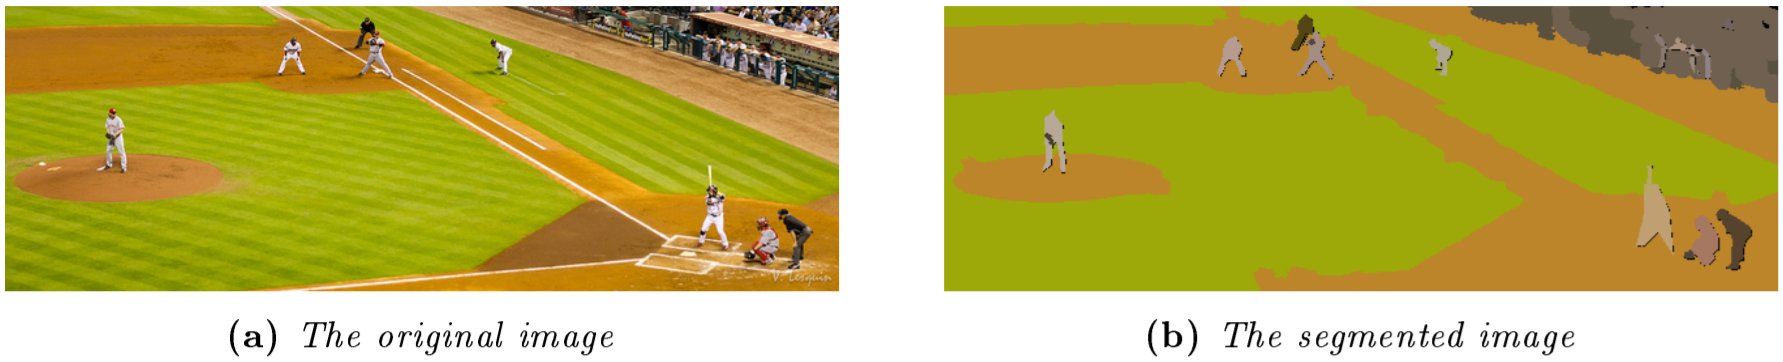
\includegraphics[width=\textwidth]{pics/segm.png}
    \caption{An image (a) and its segmented image (b).}
\end{figure}

\begin{itemize}
    \item \textbf{context:} image perception
    \item \textbf{idea:} partitioning an image into groups of similar pixels
\end{itemize}
\end{frame}
\subsection{Superpixels}
\begin{frame}{Superpixels}
\begin{figure}
    \centering
    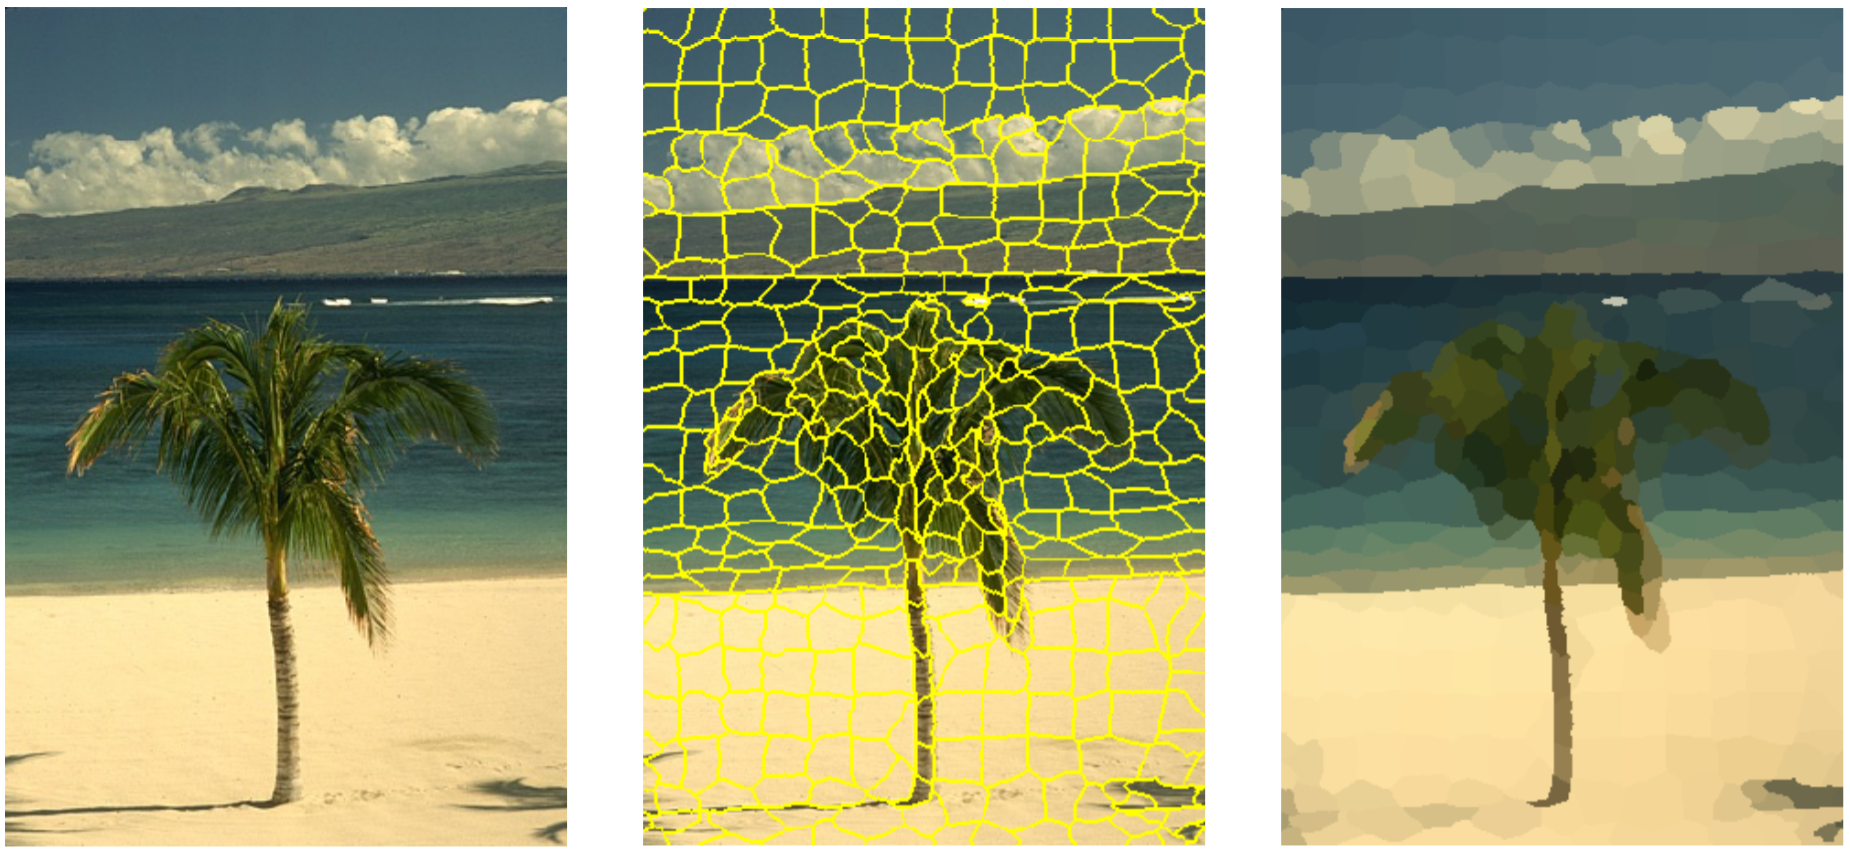
\includegraphics[width=.9\textwidth]{pics/spp.png}
    \caption{Example of a superpixel segmentation. From left to right: original image, original image with its calculated superpixels outlines and resulting superpixel segmentation in average color representation.}
\end{figure}

\begin{itemize}
    \item \textbf{idea:} over-segmentation of an image
    \item the superpixels segmentation is \textit{not unique}
\end{itemize}
\end{frame}
\subsection{Superpixels segmentation}
\begin{frame}{Superpixels metrics}
    \begin{itemize}
        \item \textbf{Boundary recall:} ratio of the number of true positive contour pixels and of the number of contour pixels in the ground truth segmentation, with a tolerance of 2 pixels

        \vspace{5mm}
        \item \textbf{Compactness:}
        $$
        \text{COMP}(S_i) = \sum_{S_i}{\frac{\mid S_i \mid}{N} \frac{4\pi A(S_i)}{P(S_i)^2}}
        $$
        \vspace{5mm}
        \item \textbf{Undersegmentation error:} Leakage of a superpixel overlapping with a gound truth segment:
        $$
        \text{UE}_{NP}(G, S) = \frac{1}{N} \sum_{G_i}{\sum_{S_j\cap G_i \neq \emptyset}{\min \left\{\mid {S_j \cap G_i} \mid, \mid {S_j - S_j \cap G_i}\mid \right\}}}
        $$
        where $S_j$ is a superpixel and $G_i$ is a ground truth segment.
    \end{itemize}
\end{frame}
\begin{frame}{Undersegmentation Error}
\begin{figure}
    \centering
    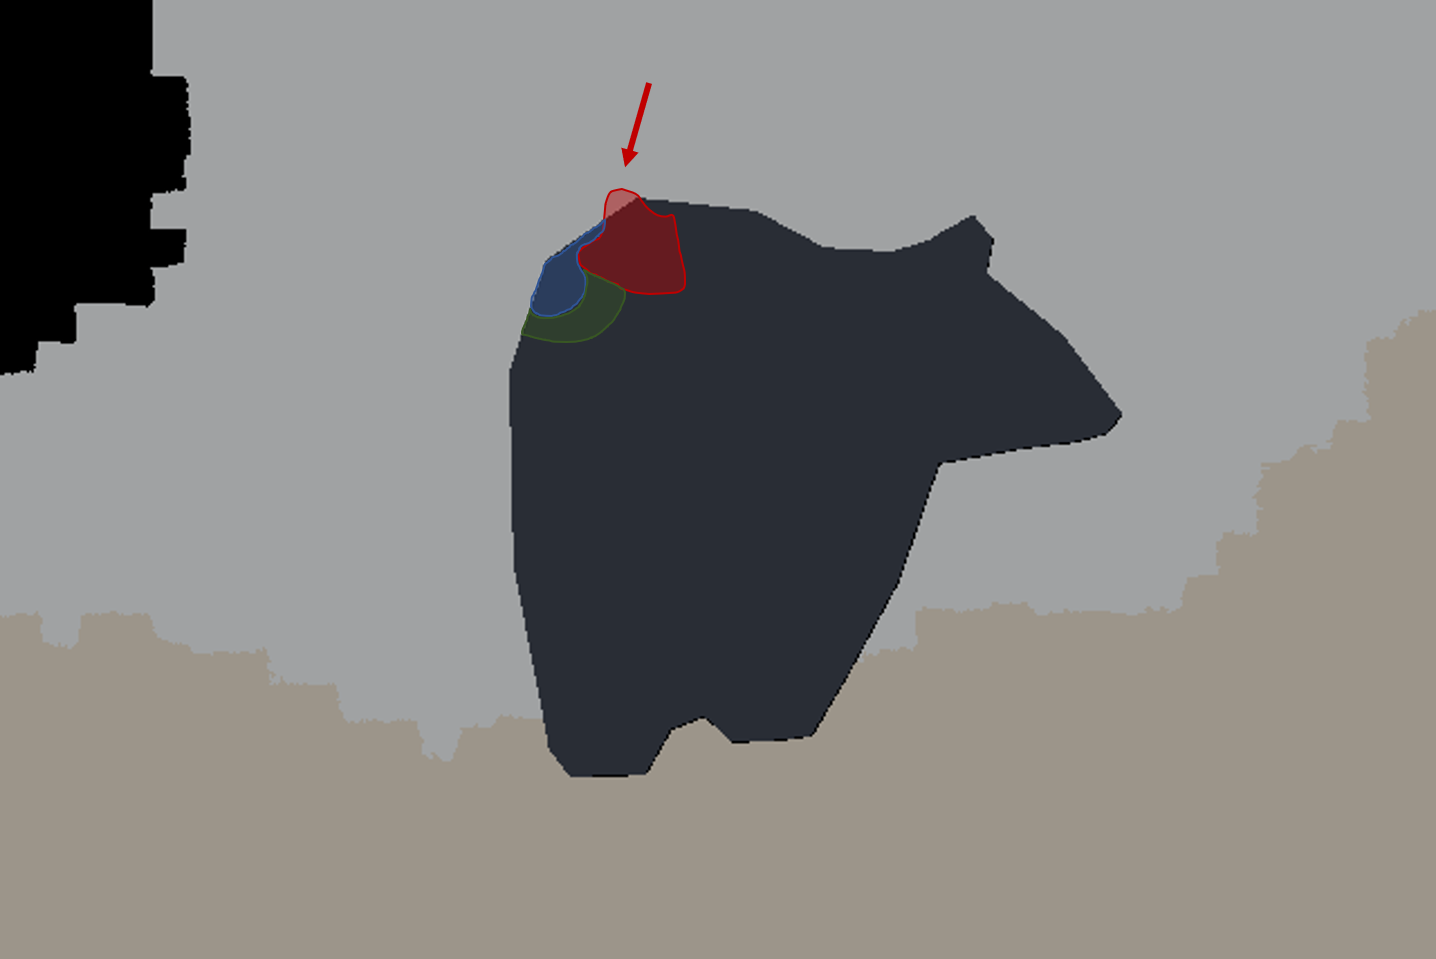
\includegraphics[width=\textwidth]{pics/underseg.png}
    \caption{Undersegmentation illustration.}
\end{figure}
\end{frame}

\subsection{Ambitions}
\begin{frame}{Ambitions}
    \begin{itemize}
        \item interest of deep learning here;
        \vspace{5mm}
        \item generating deep learning based over-segmentations? lack of proper training datasets;
        \vspace{5mm}
        \item use a CNN to improve SOTA.
    \end{itemize}
\end{frame}
\section{Dataset generation}
\subsection{Eikonal}
\begin{frame}
    \begin{figure}
    \centering
    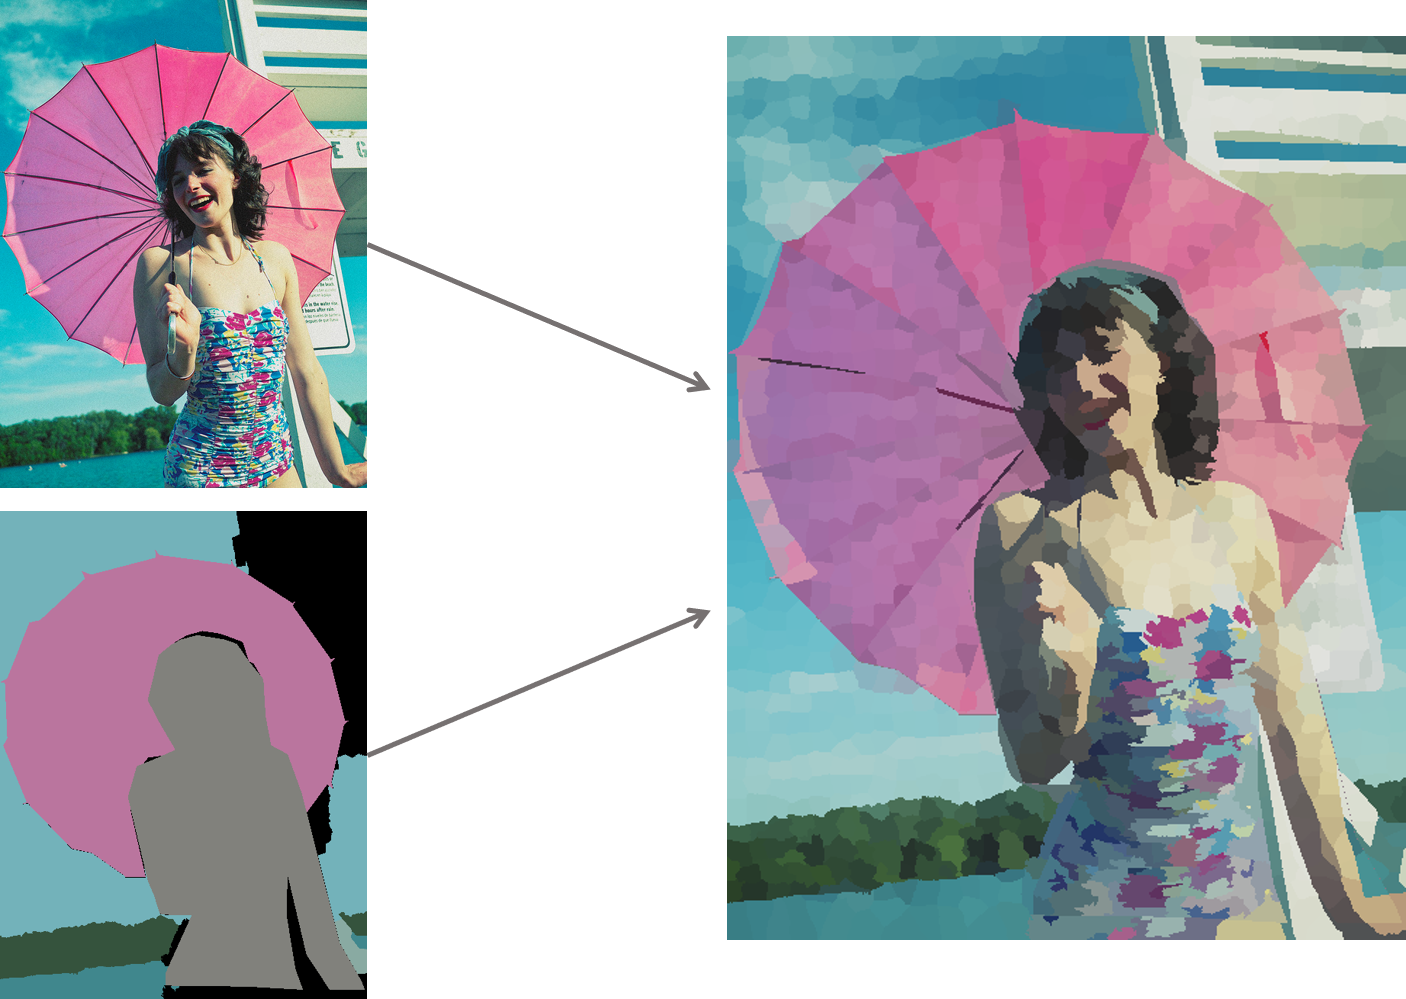
\includegraphics[width=.7\textwidth]{pics/eikonal.png}
    \caption{Eikonal algorithm principle\footnote{\textit{cf.} [1], \textit{Fast Marching Based Superpixels Generation}, Kaiwen Chang and Bruno Figliuzzi, 2019.}.}
    \end{figure}
\end{frame}
\subsection{Training}
\begin{frame}{Training}
\begin{figure}
    \centering
    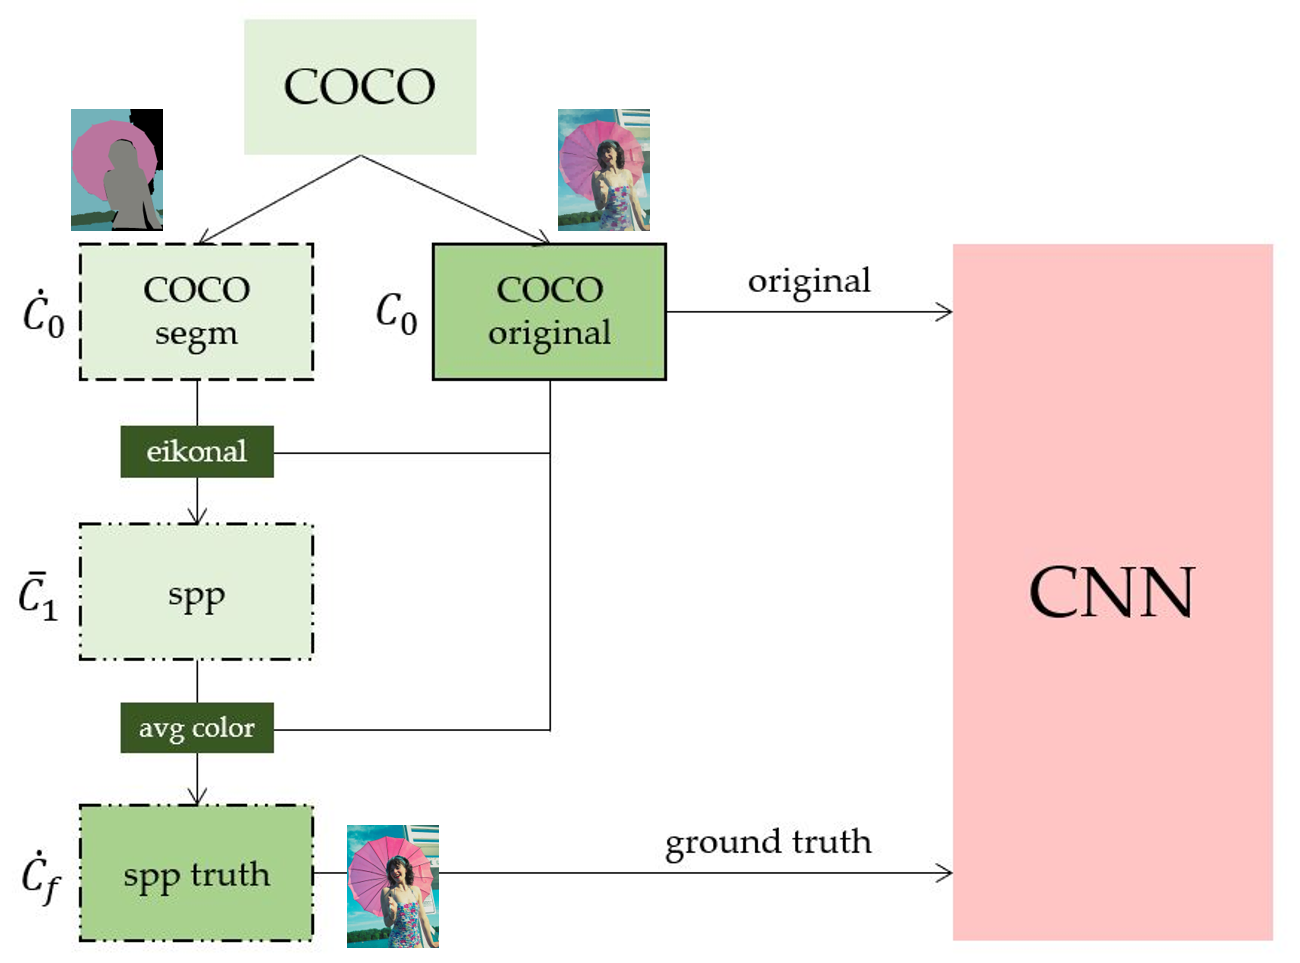
\includegraphics[width=0.9\textwidth]{pics/schema-train-img.png}
    \caption{Training process using the COCO dataset\footnote{\textit{cf.} [2], \textit{Microsoft COCO: Common Objects in Context}, \texttt{http://cocodataset.org}, 2014.}.}
\end{figure}

\end{frame}

\section{Network Architecture}
\subsection{Model}
\begin{frame}{Model Architecture: CAN}
Context Aggregation Network (CAN)\footnote{\textit{cf.} [3], \textit{Fast Image Processing with Fully-Convolutional Networks}, Qifeng Chen, Jia Xu and Vladlen Koltun, 2017.}
\begin{table}[!ht]
    \centering
    \begin{tabular}{ccccccc}
        \hline
         & $L^1$ & & $L^2$ & & $L^d=L^7$ & \\
        $m\times n\times 3$ & $\longrightarrow$ &$m\times n\times 24$ & $\longrightarrow$ & \dots & $\longrightarrow$ & $m\times n\times 3$ \\
        \hline
    \end{tabular}
    \caption{\textit{Layers of the network}}
\end{table}
For each layer:
\begin{enumerate}
    \item dilated convolution
    \item Adaptative Batch Normalization (ABN)
    \item Leaky Rectified Linear Unit (LReLU)
\end{enumerate}
\end{frame}

\begin{frame}{Dilated convolutions}
\begin{figure}
    \begin{subfigure}{.4\linewidth}
        \centering
        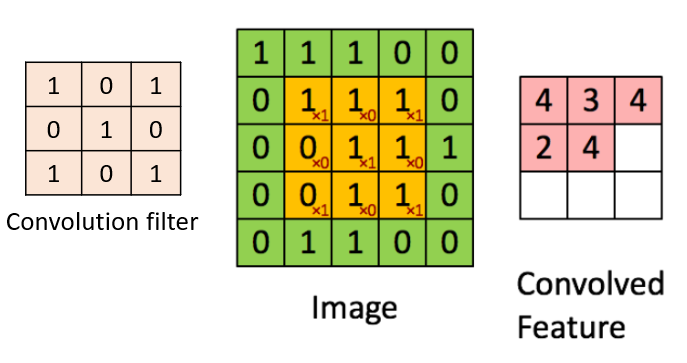
\includegraphics[width=\linewidth]{pics/conv1.PNG}
    \end{subfigure}
    \hspace{5mm}
    \begin{subfigure}{.5\linewidth}
        \centering
        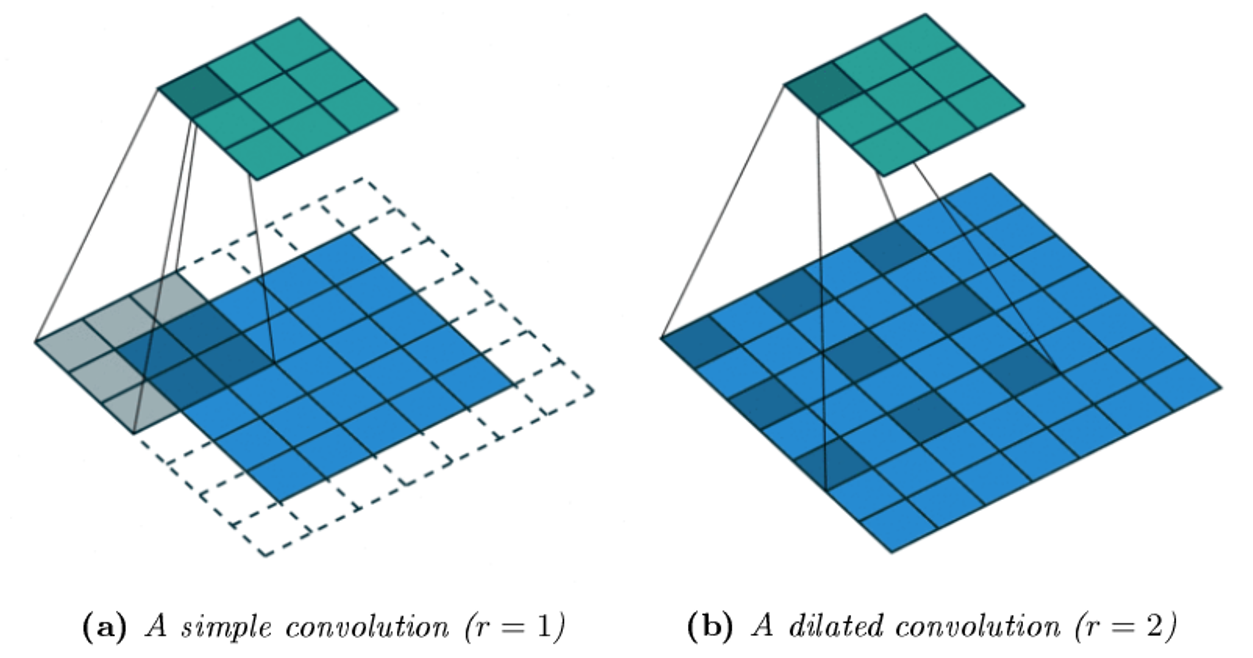
\includegraphics[width=\linewidth]{pics/dilated.png}
    \end{subfigure}
\caption{Simple and dilated convolutions.}
\end{figure}

\begin{itemize}
\item The output $C(x)$ of a pixel $x$ is:
    \begin{align*}
    C(x):& = (L_j*_r K_{i,j})(x) \\
         & = \sum_{a+rb=x}L_j(a)K_{i,j}(b) \\
         & = \sum_b L_j(x-rb)K_{i,j}(b)
    \end{align*}
\item exponential growth: global information aggregation
\end{itemize}
\end{frame}

\begin{frame}{ABN and LReLU}

\textbf{ABN}\\
\textit{Adaptive normalization function} $\Psi$:
    $$\Psi(x)=a\ x+b\ BN(x),$$
where $BN$ is the classic batch normalization, defined as:
    $$BN(x) = \frac{x-\mathrm{E}[\text{batch}]}{\sqrt{\mathrm{Var}[\text{batch}]+\epsilon}}*\gamma+\beta.$$

\textbf{LReLU}\\
$$\Phi(x)=\max(\alpha x,x)\mbox{, with } 0<\alpha<1.$$
\begin{figure}[!ht]
    \begin{subfigure}{.4\linewidth}
        \centering
        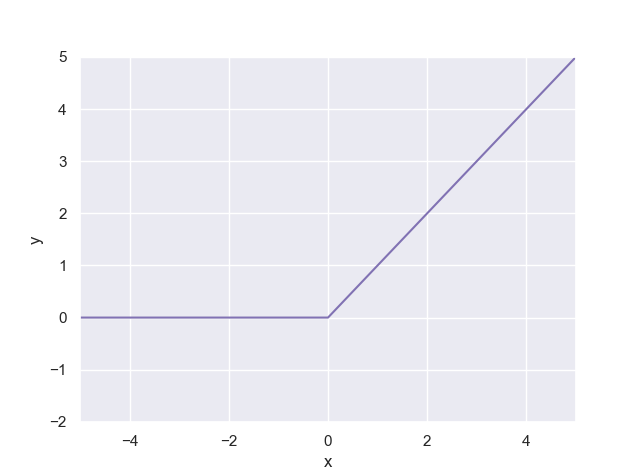
\includegraphics[width=\linewidth]{pics/act-relu.png}
        \caption{ReLU}
    \end{subfigure}
    \begin{subfigure}{.4\linewidth}
        \centering
        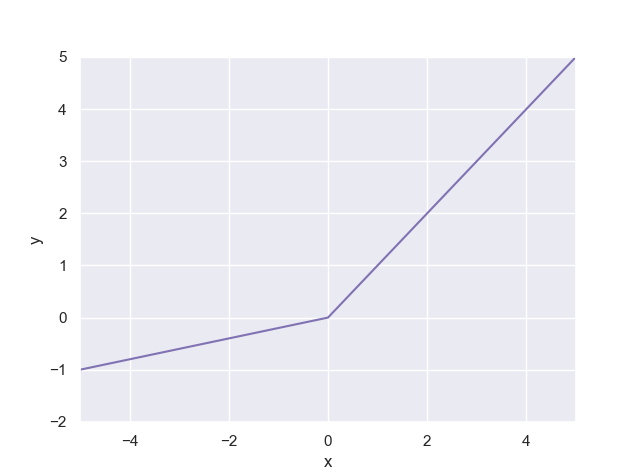
\includegraphics[width=\linewidth]{pics/act-lrelu.png}
        \caption{LReLU ($\alpha=0.2$)}
    \end{subfigure}
\end{figure}
\end{frame}

\begin{frame}{Model Architecture: CAN}
\begin{equation*}
    L_i^s=\Phi\left(\Psi^s\left(b_i^s+\sum_jL_j^{s-1}*_{r_s}K^s_{i,j}\right)\right)
\end{equation*}
\begin{table}[!ht]
    \centering\scriptsize
    \begin{tabular}{|c|c||c|cccc|cc|}
        \hline
        \multicolumn{2}{|c||}{Layer $L_s$} & 1 & 2 & 3 & 4 & 5 & 6 & 7 \\
        \hline
        \hline
         & Input $w_s$ & 3 & 24 & 24 & 24 & 24 & 24 & 24 \\
         & Output $w_{s+1}$ & 24 & 24 & 24 & 24 & 24 & 24 & 3 \\
        \cline{2-9}
        Conv & Receptive field & $\ 3\times 3\ $ & $\ 3\times 3\ $ & $\ 3\times 3\ $ & $\ 3\times 3\ $ & $\ 3\times 3\ $ & $\ 3\times 3\ $ & $\ 1\times 1\ $ \\
         & Dilation $r_s$ & 1 & 2 & 4 & 8 & 16 & 1 & 1 \\
         & Padding & 1 & 2 & 4 & 8 & 16 & 1 & 0 \\
        \hline
        \multicolumn{2}{|c||}{ABN} & Yes & Yes & Yes & Yes & Yes & Yes & Yes \\
        \hline
        \multicolumn{2}{|c||}{LReLU} & 0.2 & 0.2 & 0.2 & 0.2 & 0.2 & 0.2 & No \\
        \hline
    \end{tabular}
    \caption{Our Context Aggregation Network}
\end{table}

\end{frame}


\subsection{Loss function}
\begin{frame}{Loss function}
\vspace{5mm}
\textbf{$L_2$ Loss}
$$
L=\frac{1}{N}\sum_{i=1}^N |\hat{f}(I)_i-f(I)_i|^2
$$
\vspace{2mm}
\begin{figure}
\centering
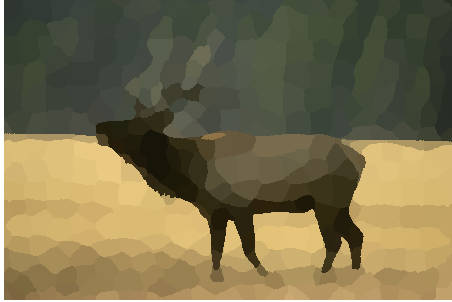
\includegraphics[width=.4\textwidth]{pics/illustration1.png}
\caption{A segmented image. Many regions have a gradient equal to $0$.}
\end{figure}
\textbf{Total Variation (TV) Loss}
$$
L_{TV}=\frac{1}{N}\sum_{i=1}^N |\hat{f}(I)_i-f(I)_i|^2+\alpha_{TV}\frac{1}{N}\sum_{i=1}^N|(\nabla f(I))_i|
$$

\end{frame}

\section{Experiments and results}
\subsection{Hyperparameters}
\begin{frame}{Experiments}


\begin{figure}[!ht]
    \begin{subfigure}{.6\linewidth}
        \footnotesize
        \begin{tabular}{|c|c|c|c|c|}
            \hline
            id & $lr_0$ & decay & thresh. & start from\\
            \hline
            \hline
            6 & $10^{-2}$ & $\times .5$ ev. 2 ep. & $10^{-4}$ & run 0 ep.5 \\
            \hline
            7 & $10^{-3}$ & \multicolumn{2}{|c|}{No} & run 0 ep.40 \\
            \hline
            8 & $10^{-2}$ & \multicolumn{2}{|c|}{No} & run 0 ep.40 \\
            \hline
            9 & $10^{-3}$ & $\times .5$ ev. 2 ep. & $10^{-4}$ & run 0 ep. 40 \\
            \hline
            10 & $10^{-3}$ & \multicolumn{2}{|c|}{No} & run 9 ep.40\\
            \hline
        \end{tabular}
        \caption{\footnotesize Runs for learning rate tuning, with $d=7$}
    \end{subfigure}
    \begin{subfigure}{.39\linewidth}
        \centering
        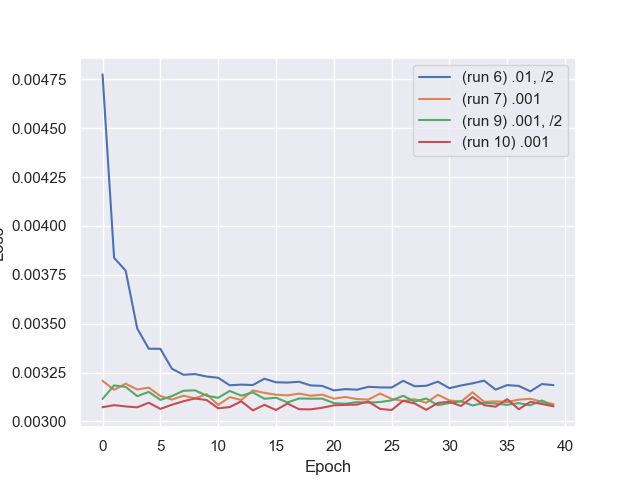
\includegraphics[width=\linewidth]{pics/hpp-lr-loss-67910.png}
        \caption{\footnotesize Runs 6, 7, 9 and 10}
    \end{subfigure}
    \caption{\footnotesize Tuning of learning rate: validation loss for different runs.}
\end{figure}

\begin{figure}[!ht]
        \centering
        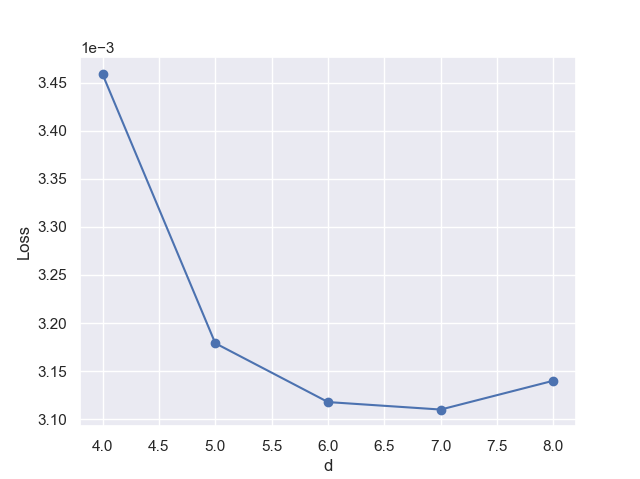
\includegraphics[width=.4\linewidth]{pics/hpp-d-8.png}
    \caption{\footnotesize Tuning of network size: loss values on the validation set.}
\end{figure}

\end{frame}
\begin{frame}{Experiments}

\begin{table}[!ht]
    \centering
    \begin{tabular}{|c|c|c|c|c|c|}
        \hline
        batch\_size & epochs & $d$ & $lr_0$ & decay for $lr_0$ & $\alpha_{TV}$ \\
        \hline
        \hline
        32 & 80 & $7$ & $10^{-2}$ & $10^{-3}$ after 10 ep. & 0 \\
        \hline
    \end{tabular}
    \caption{Hyperparameter values}
\end{table}

\end{frame}

\subsection{Results}
\begin{frame}{Testing}
\begin{figure}
    \centering
    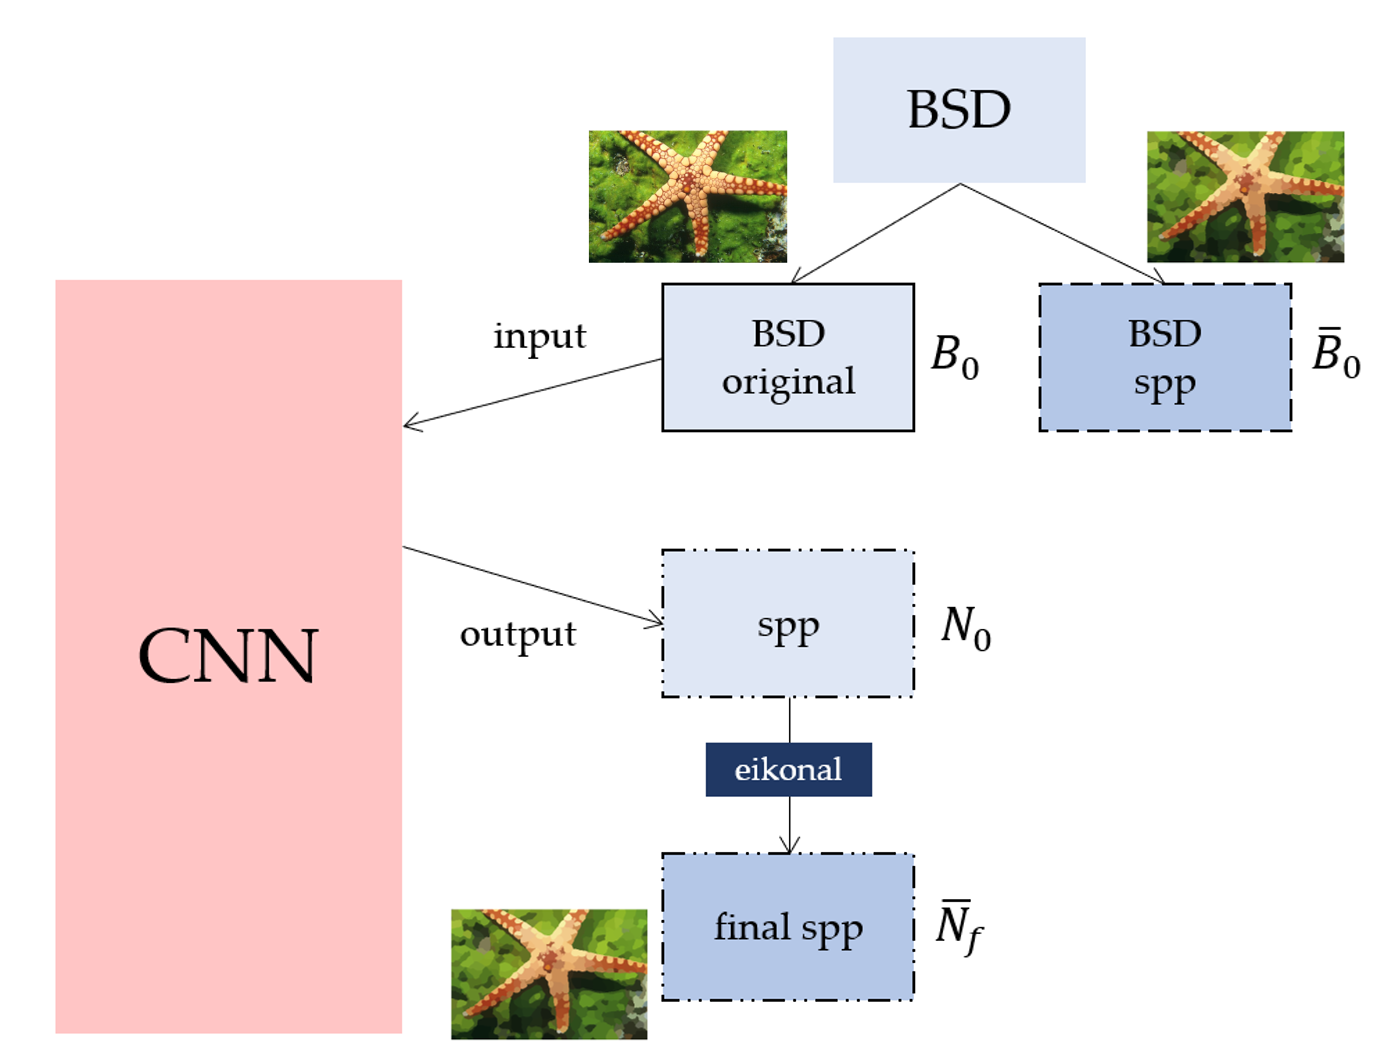
\includegraphics[width=0.9\textwidth]{pics/schema-test-img.png}
    \caption{Testing process.}
\end{figure}

\end{frame}
\begin{frame}{Results}
\begin{figure}[!ht]
    \centering
    \begin{subfigure}{.45\linewidth}
        \centering
        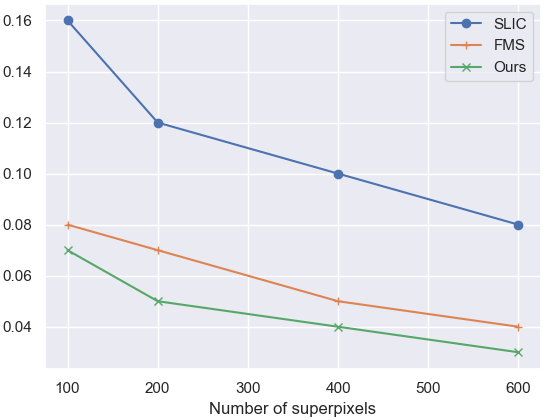
\includegraphics[width=.8\linewidth]{pics/UE.png}
    \caption{Undersegmentation Error}
    \end{subfigure}
    \begin{subfigure}{.45\linewidth}
        \centering
        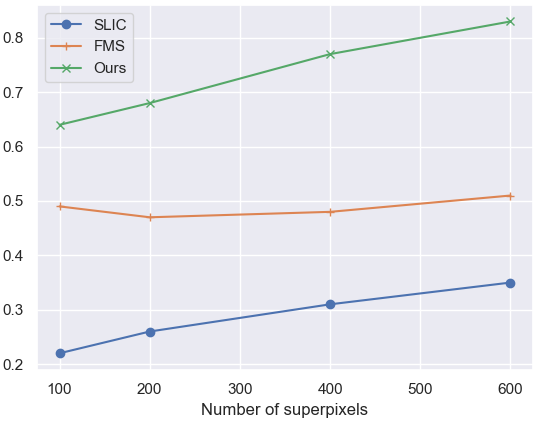
\includegraphics[width=.8\linewidth]{pics/CO.png}
    \caption{Compactness}
    \end{subfigure}
    \begin{subfigure}{.45\linewidth}
        \centering
        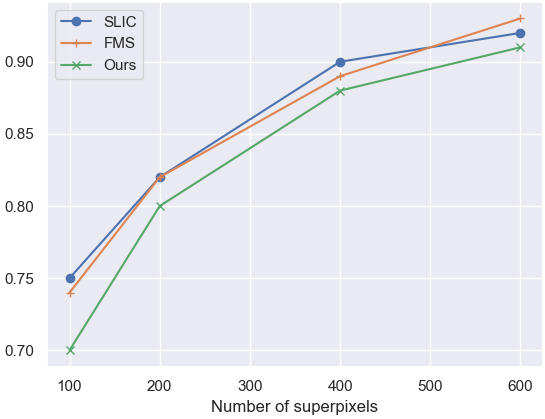
\includegraphics[width=.8\linewidth]{pics/BR.png}
    \caption{Boundary Recall}
    \end{subfigure}
    \caption{Comparisons of metrics on the BSDS500 dataset\footnote{\texttt{https://www2.eecs.berkeley.edu/Research/Projects/CS/vision/grouping/resources.html}.}}
\end{figure}
\end{frame}

\section{Discussion}
\begin{frame}{Discussion}
\begin{itemize}
    \item CNN can achieve good performance on superpixel segmentation
    \item discussion on TV-loss
        \begin{figure}
        \centering
        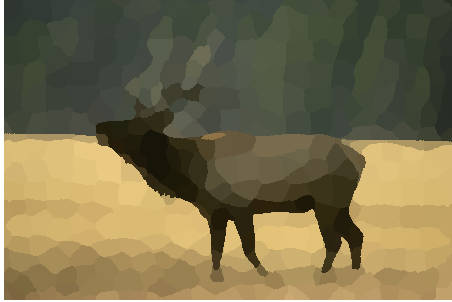
\includegraphics[width=.3\textwidth]{pics/illustration1.png}
        \end{figure}
    \item U-Net
    \item COCO dataset lacks quality
        \begin{enumerate}
            \item train on COCO and finetune on BSD?
            \item add gaussians to each superpixel?
            \item pre-process image with grid?
        \end{enumerate}
        \begin{figure}
        \centering
        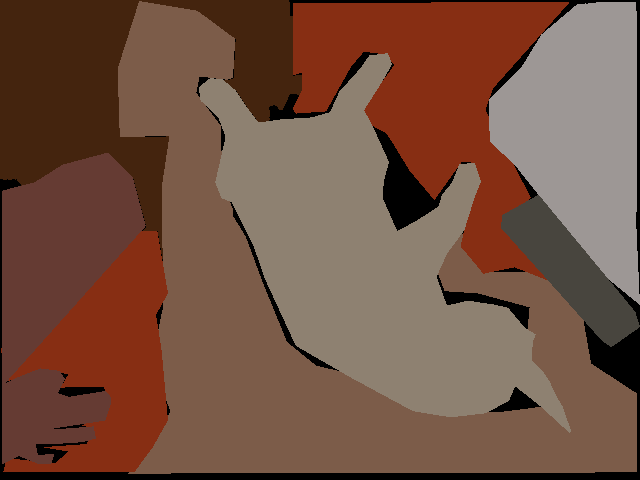
\includegraphics[width=.2\textwidth]{pics/img_segm_coco.png}
        \end{figure}
    \item application in research in grainy materials imaging, with indicator of the center of the particules
\end{itemize}
\end{frame}

\begin{frame}{Thank you}
\textbf{Essential References}
    \begin{enumerate}
        \item[] $[1]$, \textit{Fast Marching Based Superpixels Generation}, Kaiwen Chang and Bruno Figliuzzi, 2019
        \item[] $[2]$, \textit{Microsoft COCO: Common Objects in Context}, \texttt{http://cocodataset.org}, 2014
        \item[] $[3]$, \textit{Fast Image Processing with Fully-Convolutional Networks}, Qifeng Chen, Jia Xu and Vladlen Koltun, 2017
        \item[] \ldots
    \end{enumerate}

\vspace{5mm}
\textbf{Code:} \texttt{github.com/theodumont/superpixels-segmentation}

\vspace{20mm}
\centering
    Thank you very much to M. Bruno Figliuzzi.
\end{frame}


\end{document}
